\documentclass[12pt,a4paper,titlepage,headinclude,bibtotoc]{scrartcl}

%---- Allgemeine Layout Einstellungen ------------------------------------------

% Für Kopf und Fußzeilen, siehe auch KOMA-Skript Doku
\usepackage[komastyle]{scrpage2}
\pagestyle{plain}
\setheadsepline{0.5pt}[\color{black}]
\automark[section]{chapter}


%Einstellungen für Figuren- und Tabellenbeschriftungen
\setkomafont{captionlabel}{\sffamily\bfseries}
\setcapindent{0em}


%---- Weitere Pakete -----------------------------------------------------------
% Die Pakete sind alle in der TeX Live Distribution enthalten. Wichtige Adressen
% www.ctan.org, www.dante.de

% Sprachunterstützung
\usepackage[ngerman]{babel}
\usepackage{caption}
% Benutzung von Umlauten direkt im Text
% entweder "latin1" oder "utf8"
\usepackage[utf8]{inputenc}

% Pakete mit Mathesymbolen und zur Beseitigung von Schwächen der Mathe-Umgebung
\usepackage{latexsym,exscale,stmaryrd,amssymb,amsmath}


\usepackage[nointegrals]{wasysym}
\usepackage{eurosym}

% Anderes Literaturverzeichnisformat
%\usepackage[square,sort&compress]{natbib}
\usepackage{hyperref}
% Für Farbe
\usepackage{color}
\usepackage{graphicx}
\usepackage{wrapfig}
\usepackage{subfigure}

% Caption neben Abbildung
\usepackage{sidecap}


% Befehl für "Entspricht"-Zeichen
\newcommand{\corresponds}{\ensuremath{\mathrel{\widehat{=}}}}
% Befehl für Errorfunction
\newcommand{\erf}[1]{\text{ erf}\ensuremath{\left( #1 \right)}}


%Fußnoten zwingend auf diese Seite setzen
\interfootnotelinepenalty=1000

%Für chemische Formeln (von www.dante.de)
%% Anpassung an LaTeX(2e) von Bernd Raichle
\makeatletter
\DeclareRobustCommand{\chemical}[1]{%
  {\(\m@th
   \edef\resetfontdimens{\noexpand\)%
       \fontdimen16\textfont2=\the\fontdimen16\textfont2
       \fontdimen17\textfont2=\the\fontdimen17\textfont2\relax}%
   \fontdimen16\textfont2=2.7pt \fontdimen17\textfont2=2.7pt
   \mathrm{#1}%
   \resetfontdimens}}
\makeatother
\usepackage{textcomp}
\usepackage{upgreek}
%\begin{document}
%$\upmu$
%\end{document}
%Honecker-Kasten mit $$\shadowbox{$xxxx$}$$
\usepackage{fancybox}

%SI-Package
\usepackage{siunitx}

%keine Einrückung, wenn Latex doppelte Leerzeile
\parindent0pt

%Bibliography \bibliography{literatur} und \cite{gerthsen}
%\usepackage{cite}
\usepackage{babelbib}
\selectbiblanguage{ngerman}

\usepackage{siunitx}
%\begin{document}
 % \SI{1.55}{\micro\metre}
\sisetup{math-micro=\text{µ},text-micro=µ}
\usepackage{amsmath}

\usepackage[verbose]{placeins}
%für \FloatBarrier

\begin{document}

\begin{titlepage}
\centering
\textsc{\Large Physikalisch- Chemisches Grundpraktikum\\[1.5ex] Universität Göttingen}

\vspace*{0.5cm}

\rule{\textwidth}{1pt}\\[0.5cm]
{\huge \bfseries
  Versuch 1: \\[1.5ex]
  Molare Wärmekapazität von Festkörpern }\\[0.5cm]
\rule{\textwidth}{1pt}

\vspace*{0.5cm}


\begin{Large}
\begin{tabular}{ll}
Durchführende: &  Isaac Maksso, Julia Stachowiak\\
Assistent: & Christoph \\
 Versuchsdatum: & 3.11.2016\\
 Datum der ersten Abgabe: & 10.11.2016\\
 Datum der zweite Abgabe: & 24.11.2016\\
\end{tabular}
\end{Large}

\vspace*{0.5cm}


\begin{table}[h!]
\centering
\caption{Ergebnisse des Versuchs.}
\begin{tabular}{c|c|c}
Probe& $<\Theta_D >$ [K]& $<\Theta_{D,Lit.}>$ [K] \\
\hline
Graphit &1326 ± 4 & 1725\\
\hline
Zink & 317$^*$ & 345\\
\hline
Kupfer & 552$^*$ &308\\
\end{tabular}
\caption*{* korrigierter Mittelwerte (siehe Diskussion).}
\end{table}
\footnotetext{Quelle: https://de.wikipedia.org/wiki/Campher, aufgerufen am 31.12.16}
 \footnotetext{Quelle: http://www.chemie.de/lexikon/Kaliumchlorid.html, aufgerufen am 31.12.16}
\end{titlepage}


\tableofcontents

\newpage


\section{Experimentelles}
\subsection{Experimenteller Aufbau}

\begin{figure} [h!]
\begin{center}
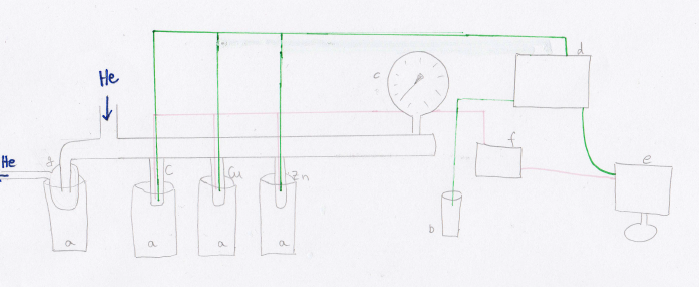
\includegraphics[scale=0.9]{VersuchsaufbauZeichnung.png} \end{center}
\caption{Versuchsaufbau.}
\end{figure}

a) Dewergefäß\\
b) Vergleichstemperaturbad ($T_{Soll}=$273,15 K)\\
c) Druckanzeige\\
d) Thermoelement\\
e) PC mit Labview\\
f) Heizsteuerung\\
g) Gasauffang\\
\subsection{Durchführung}
Die Messung erfolgte für jeden Stoff bei Zimmertemperatur, in einem Stickstoffbad und in einem Stickstoff/Ethanolbad und einem Heizstrom von 750~mA. Zur Einstellung einer festen Temperatur wurde Helium durch die Apparatur geleitet und anschließend mittels Vakuum wieder abgezogen, um die Probeen thermisch zu isolieren. Die Messung war in Vorlaufphase (60~s), Heizphase (20~s) und Endphase (200~s) unterteilt. Während der Heizphase wurde ein Heizstrom (750~mA) zugeführt und die auftretende Thermospannung inklusive Änderung (Fehler) mittels eines Thermoelements notiert. Die Temperatur wurde mit einem Eisbad als Referenz mit dem Programm "Labview$"$ aufgezeichnet.\\
\section{Auswertung}
\subsection{Messergebnisse}
In der Tabelle 1 sind die Messergebnisse der Heizspannung sowie der Temperaturdifferenz dargestellt.
\begin{table}[h!]
\centering
\caption{Messergebnisse des Versuchs.}
\begin{tabular}{c|c|c|c|c|c|c}
&\multicolumn{2}{c}{RT}&\multicolumn{2}{|c}{$\text{N}_2$/EtOH}&\multicolumn{2}{|c}{$\text{N}_2$}\\
\hline
&$\Delta T$/\;K&  U/\;V&$\Delta T$/\;K&  U/\;V&$\Delta T$/\;K&  U/\;V\\
\hline
Graphit & 4 & $3,22\pm0,01$ & 4,1 &$3,20\pm0,03$&4,6&$3,16\pm0,05$\\  
Kupfer & 1,2 & $3,72\pm0,02$ & 1 &$3,68\pm 0,01$&0,8&$3,61\pm0,03$\\ 
Zink & 1,4 & $3,61\pm 0,02$ &1 &$3,53\pm0,04$&0,8&$3,53\pm 0,09$ \\ 
\end{tabular} 
\end{table}
\FloatBarrier
\subsection{Bestimmung von $f$}

Die experimentell ermittelte molare Wärmekapazität bei konstantem Druck errechnet sich folgendermaßen:\\

\begin{equation}
c_{m,p} = \frac{UI\Delta t}{n\Delta T}
\end{equation}

Hierbei wurde ein Heizstrom $I$ von 750~mA und eine Heizzeit $\Delta t$ von 20~s eingestellt. Die Auswertungsergebnisse sind in der Tabelle 2 aufgelistet.
\begin{table}[h!]
\centering
\caption{Ergebnisse für $\text{c}_P^{\text{Exp.}}$.}
\begin{tabular}{c|c|c|c|c}
Probe& Spannungsabfall [V] & $\Delta$T [K]& Stoffmenge [mol] &  $\text{c}_P^{\text{Exp.}}$ [$\frac{\text{J}}{\text{mol}\cdot\text{K}}$]\\
\hline
Graphit & 3,22&4 &2,67 &4,52 \\
\hline
Kupfer & 3,72 & 1,2&0,900&51,7  \\
\hline
Zink & 3,61& 1,4& 0,692 &55,9\\
\end{tabular}
\end{table}
\FloatBarrier 

Der Korrekturfaktor \textit{f} ergibt sich aus dem Verhältnis von $\text{c}_P^{\text{Lit.}}$und $\text{c}_P^{\text{Exp.}}$. Die Korrekturfaktorenfür Graphit, Kupfer und Zink sind in Tabelle 3 dargestellt. 
\begin{equation}
f=\frac{\text{c}_P^{\text{Lit.}}}{\text{c}_P^{\text{Exp.}}}
\end{equation}
\begin{table}[h!]
\centering
\caption{Ergebnisse für $f$.}
\begin{tabular}{c|c|c}
Probe&$\text{c}_P^{\text{Lit.}}$ [$\frac{\text{J}}{\text{mol}\cdot\text{K}}$]&$f$\\
\hline
Graphit &8,517 &1,88 \\
\hline
Kupfer& 24,47&0,474  \\
\hline
Zink & 25,330&0,453\\
\end{tabular}
\end{table}
\FloatBarrier

Die Messgrößen des Spannungsabfalls, Heizstroms und der Temperatur sind fehlerbehaftet. Es wurde eine Gaussische Fehlerfortpflanzung aufgestellt um $\Delta\text{c}_P^{\text{Exp.}}$, $\Delta f$ und $\Delta\text{c}_P^{\text{Neu}}$ zu bestimmen:
\begin{align}
\Delta \text{c}_P^{\text{Exp.}}&=\sqrt{ \left(\frac{I\Delta t}{n\Delta T}\cdot \Delta U \right)^2+\left(\frac{U\Delta t}{n\Delta T}\cdot \Delta I \right)^2+\left(- \frac{I\Delta t}{n\Delta T^2}\cdot \Delta\Delta T\right)^2}\\
\Delta \text{c}_P^{\text{Exp.}}(\text{Graphit bei ZT})&=\Biggl( \left(\frac{750\cdot 10^{-3}\;\text{A} \cdot 20\;\text{s}}{2,67\;\text{mol}\cdot 4\;\text{K}}\cdot 0,01\;\text{V} \right)^2+\left(\frac{3,22\;\text{V} \cdot 20\;\text{s}}{2,67\;\text{mol}\cdot 4\;\text{K}}\cdot750\cdot 10^{-5}\;\text{A} \right)^2\\
& +\left(\frac{750\cdot 10^{-3}\;\text{A} \cdot 20\;\text{s}}{2,67\;\text{mol}\cdot (4\;\text{K})^2}\cdot 0,05\;\text{K} \right)^2\Biggr)^{\frac{1}{2}}\\
&=0,46 \;\frac{\text{J}}{\text{mol}\cdot\text{K}}
\end{align}
\begin{table}[h!]
\centering
\caption{Ergebnisse für $\Delta \text{c}_P^{\text{Exp.}}$.}
\begin{tabular}{c|c|c|c}
Probe&Temperaturbad&$\Delta U$ [V]&$\Delta \text{c}_P^{\text{Exp.}}$ [$\frac{\text{J}}{\text{mol}\cdot\text{K}}$]\\
\hline
Graphit& Zimmertemperatur&0,01&0,46\\
\hline
&Stickstoff&0,01&0,21\\
\hline
&Stickstoff/Ethanol&0,01&0,44\\
\hline
Kupfer&Zimmertemperatur&0,02& 5,6\\
\hline
&Stickstoff&0,01&8,9\\
\hline
&Stickstoff/Ethanol&0,01&6,9\\
\hline
Zink &Zimmertemperatur&0,02& 5,9\\
\hline
&Stickstoff&0,01&11\\
\hline
&Stickstoff/Ethanol&0,01&8,6\\
\end{tabular}
\end{table}
\FloatBarrier
Die Ungenauigkeit des Korrekturfaktors $\Delta f$ ergibt sich ebenfalls aus der Fehlerfortpflanzung:
\begin{align}
\Delta f &= \sqrt{ \left(-\frac{\text{c}_P^{\text{Lit.}}}{(\text{c}_P^{\text{Exp.}})^2}\cdot \Delta \text{c}_P^{\text{Exp.}} \right)^2}\\
\Delta f (\text{Graphit})&= \sqrt{ \left(-\frac{8,517\;\frac{\text{J}}{\text{mol}\cdot\text{K}}}{(4,52\;\frac{\text{J}}{\text{mol}\cdot\text{K}})^2}\cdot 0,014\;\frac{\text{J}}{\text{mol}\cdot\text{K}}\right)^2}\\
&= 0,006\\
\Delta f (\text{Zink})&=0,003\\ 
\Delta f (\text{Kupfer})&=0,003\\
\end{align} 
$\Delta\text{c}_P^{\text{Neu}}$ wurde folgendermaßen berechnet:
\begin{align}
\Delta\text{c}_P^{\text{Neu}}&= |\frac{\partial\Delta\text{c}_P^{\text{Neu}}}{\partial \text{c}_P^{\text{Exp.}}} \cdot \Delta\text{c}_P^{\text{Exp.}} |+ |\frac{\partial\Delta\text{c}_P^{\text{Neu}}}{\partial f} \cdot \Delta f|\\
&=| f \cdot \Delta\text{c}_P^{\text{Exp.}}| + |\text{c}_P^{\text{Exp.}} \cdot \Delta f |
\end{align} 
Die Ergebnisse der korrigierten Wärmekapazitäten sind in der Tabelle 5 dargestellt.
\begin{table}[h!]
\centering
\caption{Ergebnisse für $\Delta\text{c}_P^{\text{Neu}}$}
\begin{tabular}{c|c|c}
Probe&Temperaturbad&$\text{c}_P^{\text{Neu}}$ [$\frac{\text{J}}{\text{mol}\cdot\text{K}}$]\\
\hline
Graphit& RT&8,5 ± 0,5 \\
\hline
&$\text{N}_2$&4,0 ± 0,2 \\
\hline
&$\text{N}_2$/EtOH&8,3 ± 0,4 \\
\hline
Kupfer &RT& 24 ± 6\\
\hline
&$\text{N}_2$& 36 ± 9\\
\hline
&$\text{N}_2$/EtOH& 29 ± 5\\
\hline
Zink &RT&25,3± 5,9\\
\hline
&$\text{N}_2$&43,3 ± 11\\
\hline
&$\text{N}_2$/EtOH& 34,7 ± 8,6\\
\end{tabular}
\end{table}
\FloatBarrier
Die berechneten $\text{c}_P^{\text{Neu}}$-Werte wurden gegen die Temperatur aufgetragen. Abbildung 2, 3 und 4 zeigen den Kurvenverlauf für Graphit, Kupfer und Zink.
\begin{figure} [h!]
\centering
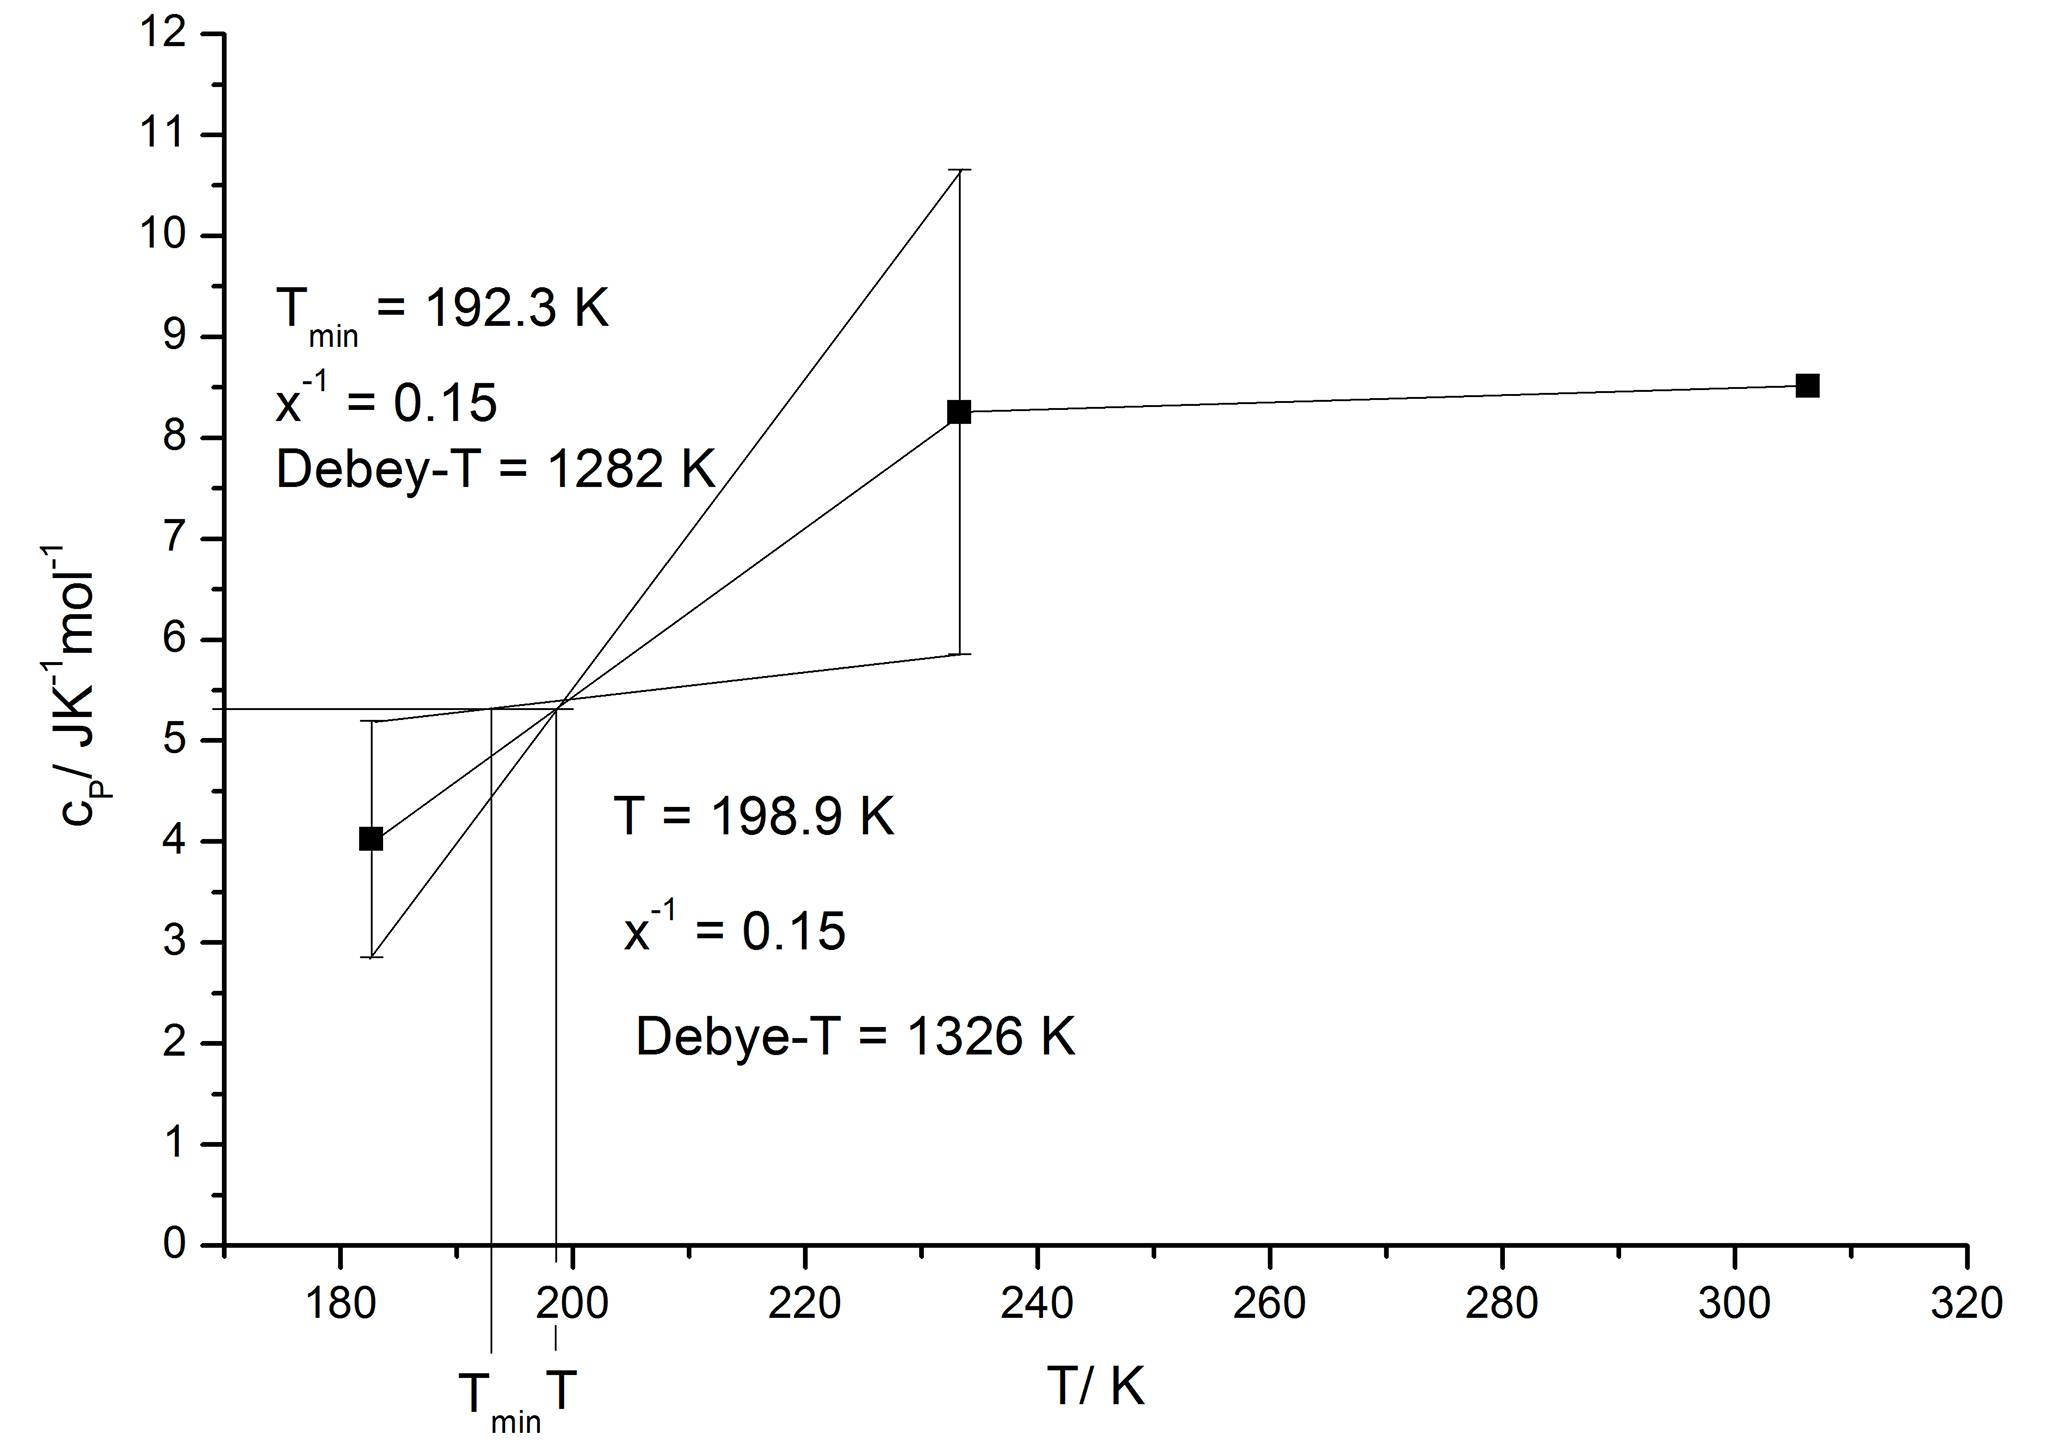
\includegraphics[width=13.5cm]{Grap_Deb.jpeg}
\caption{$c_p(T)$ Graphit.}
\end{figure} 
\FloatBarrier

\begin{figure} [h!]
\centering
\includegraphics[width=13.5cm]{Kupfer_ja.jpeg} 
\caption{$c_p(T)$ Kupfer.}
\end{figure} 
\FloatBarrier  

\begin{figure} [h!]
\centering
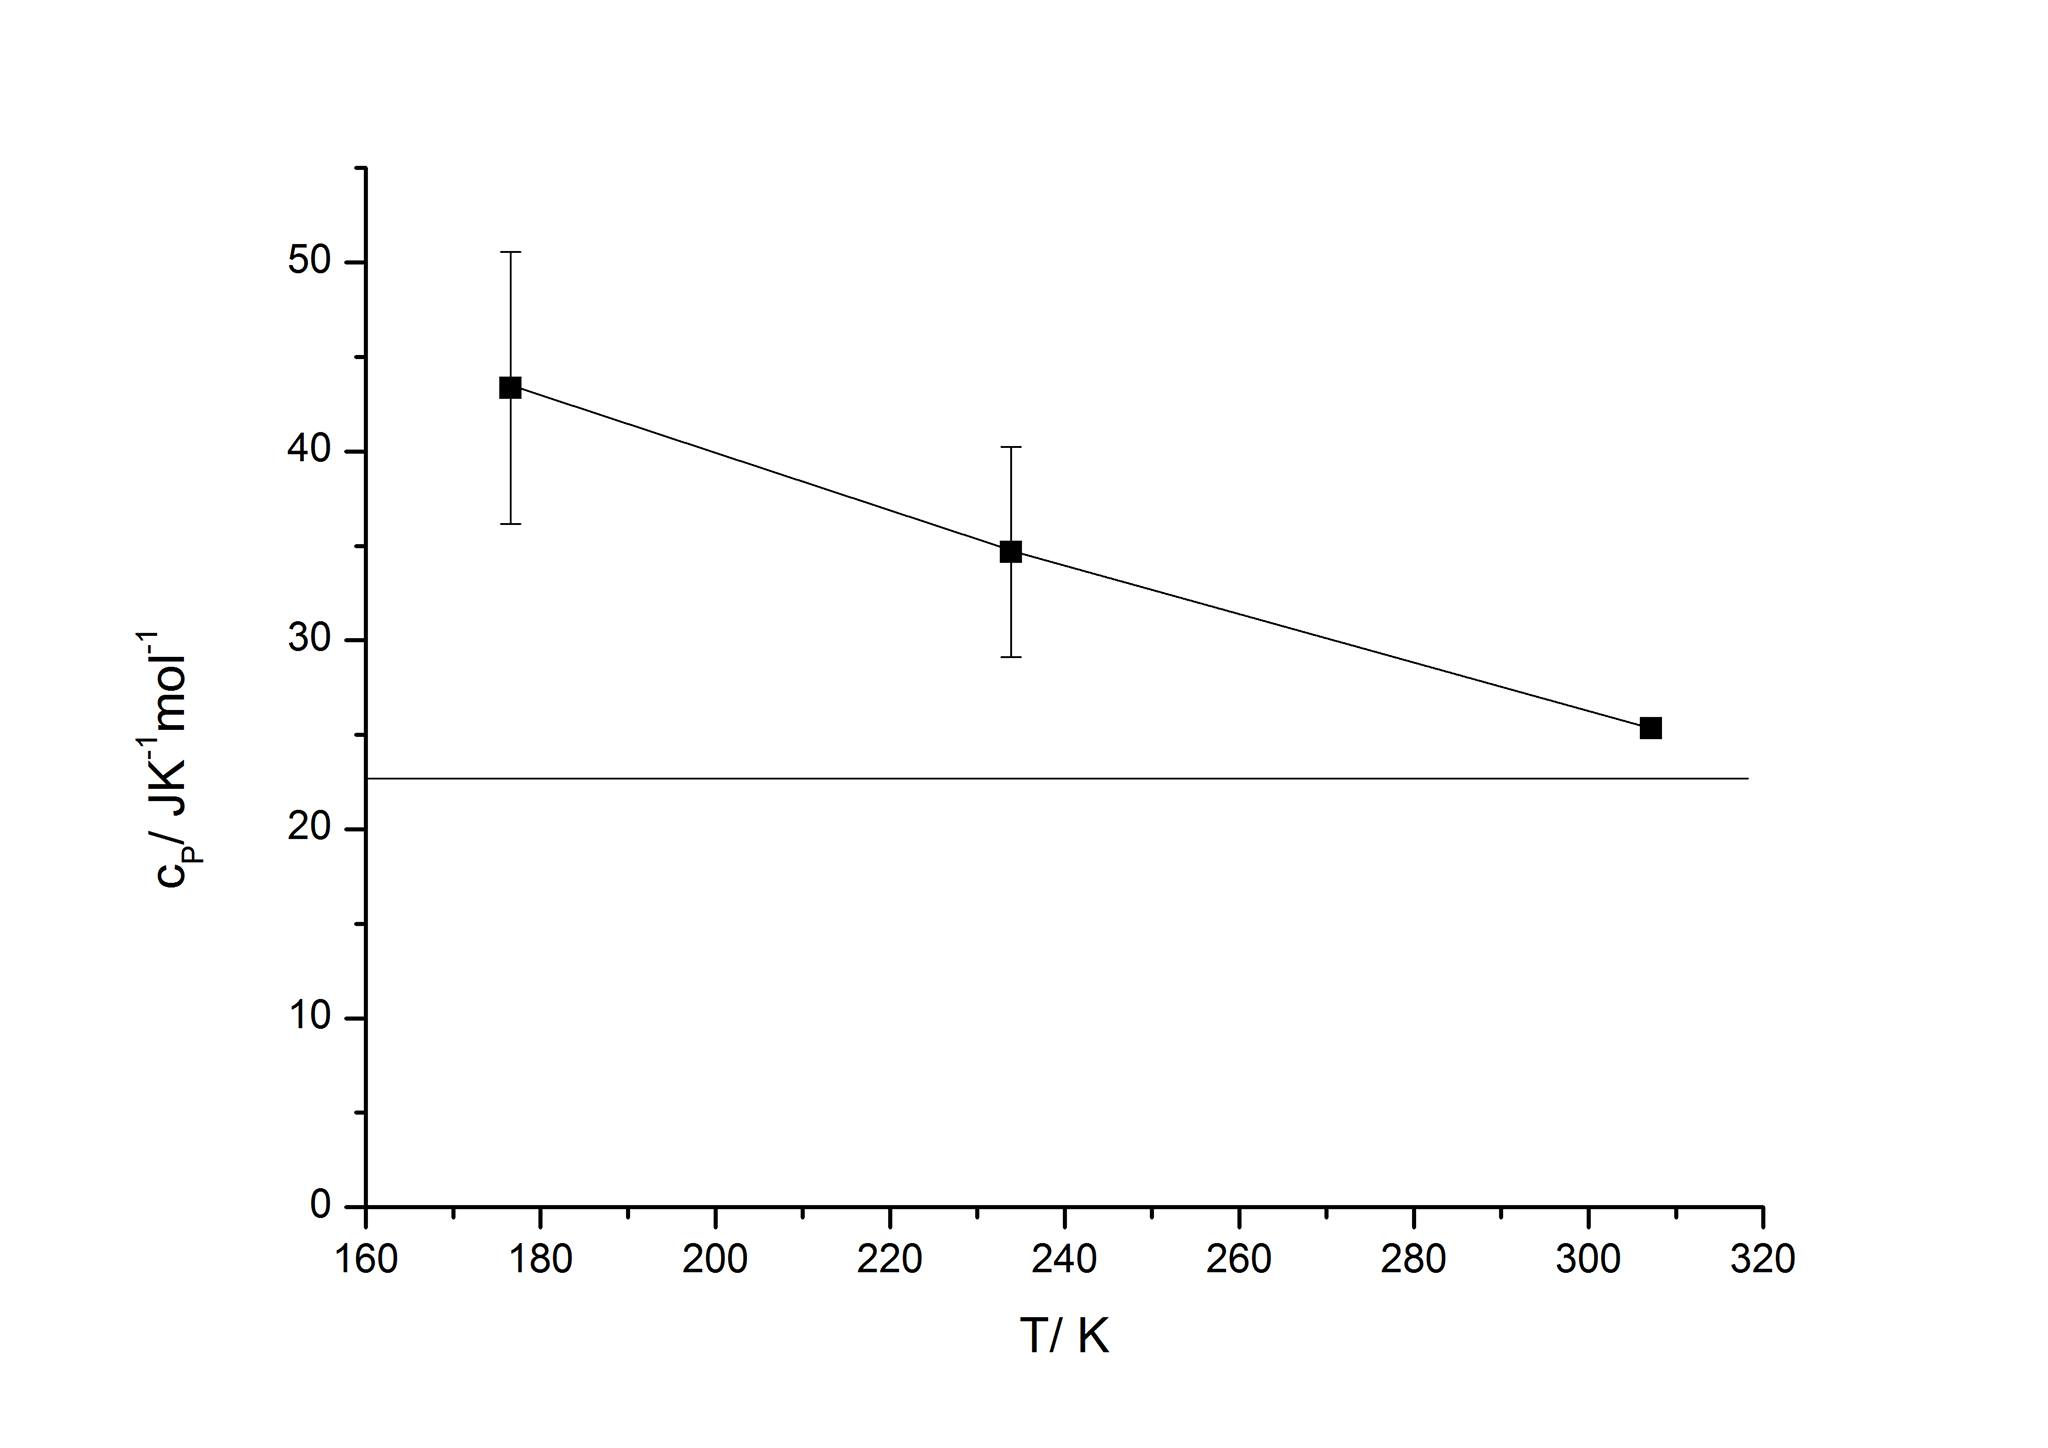
\includegraphics[width=13.5cm]{Zink_ja.jpeg} 
\caption{$c_p(T)$ Zink.}
\end{figure}    
\FloatBarrier 

%\begin{table} [h] 
%\centering
%\caption{Werte zur linearen Interpolation}
%\begin{tabular} {r | r|  r }
%& Steigung $m$& Schnittpunkt mit Ordinate $n$\\
%\hline
%Graphit& 0,00512&3,0229\\
%Cu&	0,0860	&-15,5\\
%Zn&	-0,422	&169\\
%\end{tabular}
%\end{table}


\subsection{Berechnung von $c_{V}(T)$ nach Debye}
Die für verschiedene $\frac{T}{\Theta_{D}}$-Verhältnisse theoretischen Wärmekapazitäten der Stoffe können mittels Debye folgendermaßen berechnet werden:\\

\begin{equation}
c_{V}(T)= 3R \cdot \left(4 D(x) - \frac{3x}{e^x -1}\right)
\end{equation}

mit \\

\begin{equation}
D(x) = \frac{3}{x^3}\cdot \int_{0}^{x} \frac{t^3}{e^t -1} dt
\end{equation}

und $x= \frac{\Theta_D}{T}$.


%nachfolgende Tabelle mit den richtigen aktualisierten Werten
\begin{table} [h]
\centering
\caption{theoretische $c_V$-Werte nach Debye}
\begin{tabular} {r | r|  r | r}
&$\frac{T}{\Theta_D}=\frac{1}{x}$& D(x)&$c_V(T)[\mathrm{J}\cdot \mathrm{mol}^{-1} \cdot \mathrm{K}^{-1}]$\\
\hline
Graphit	&0,15&	0,0596	&5,31\\
	&0,2&	0,118	&9,20\\
	&0,25	&0,182&	12,5\\
	&0,3	&0,244	&15,2\\
	\hline			
Cu/Zn &	0,4	&0,354&	18,6\\
	&0,5&	0,441	&20,6\\
	&0,6	&0,510	&21,8\\
	&0,7&	0,564&22,6\\

\end{tabular}
\end{table}

\FloatBarrier
\subsection{Berechnung der zugehörigen $<\Theta_D>$-Werte }
Die Debye-Temperatur wurde graphisch ermittelt. Hierzu wurde die $c_V$-Werte aus 2.3 in die Graphen eingesezeichnet und der x-Achsenabschnitt bestimmt. Dieser Wert wurde mit dem reziproken Wert von x multipliziert, um die Debye-Temperatur zu erhalten. Es konnte nur die Debye-Temperatur des Graphits bestimmt werden, da keine $c_V$-Werte bei Zink und Kupfer den Graphen schneiden.
\begin{align}
T_{\text{Graphit}} &= 198.9\;\text{K}\\
\Theta_{D, \text{Graphit}} &= \frac{T_{\text{Graphit}}}{x}\\
&= \frac{198,9\;\text{K}}{0,15}\\
&= 1326\;\text{K}
\end{align}
Der Fehler wurde graphisch mittels Grenzgeraden ermittelt. Da die $T_{max}$ sehr ähnlich der Temperatur $T_{\text{Graphit}}$ ist, wurde $T_{\text{Graphit}}$ als $T_{max}$ angenommen. 
\begin{align}
\Delta T&= \frac{|T_{max} - T_{min}|}{2} \\
&= \frac{|(198.9-192.3)\;\text{K}|}{2}\\
&= 3,3\;\text{K}
\end{align}
%\subsection{Berechnung der zugehörigen $<\Theta_D>$-Werte }


%Für Festkörper gilt: $c_V =c_p -R$, so kann die Gleichung auch auf die soben aus den Debye-Temperaturen ermittelten theoretischen $c_V(T)$-Werte angewendet werden. Somit können die zu den $c_V$-Werten zugehörigen Temperaturwerte ermittelt werden:\\

%\begin{equation}
%T= \frac{c_V(T) -n +R}{m}
%\end{equation}

%Zu den so errechneten Temperaturen werden die zugehörigen Debye-Temperaturen ermittelt nach:\\

%\begin{equation}
%T \cdot x = \Theta_D
%\end{equation}

%Letztendlich ergeben sich daraus folgende $\Theta_D$-Mittelwerte:\\


%aktualisierte Werte in dieser Tabelle 09.11.16
%\begin{table} [h]
%\centering
%\caption{$<\Theta_D>$ für jeweiliges Material}
%\begin{tabular} {r | r|  r |r |r}
%& $c_V$ [J/mol K] & T	[K] &$\Theta_D$ [$10^2\cdot$K]	&$<\Theta_D>$ [K]\\
%\hline
%Graphit &5,31	&2071	&138&	138$\cdot10^2$\\
   %     &9,20	&28,3&	141\\	
      %  &12,5&	34,8&	139\\	
      %  &15,1	&40,0	&133\\
%\hline						
%Cu &18,6 &	494 &	123$\cdot 10^1$ &	981\\
%&20,6 &	517&	103 $\cdot 10^1$&\\
%&21,8&	531 &	885& \\
%&22,6 &	540 &	771&\\	
%\hline			
%Zn &18,6 &	336 &	841 &	630  \\
%&20,6 &	332 &	663&  \\	
%&21,8 &	329 &	548& \\	
%&22,6 &	327& 	467& \\

%\end{tabular}
%\end{table}

\subsection{Auftragung $\frac{T}{\Theta_D}$}
Bei Festkörpern ist $c_V \approx c_P$. In Tabelle\;8 sind die Werte zur Auftragung $c_V$ gegen $\frac{T}{\Theta_D}$ dargestellt. 
%die Werte mussten nicht aktualisiert werden
\begin{table} [h]
\centering
\caption{Werte zur Auftragung von $c_V$ nach 2.2 gegen $\frac{T}{\Theta_D}$}
\begin{tabular} {r | r |r | r }
&$\Theta_{D,Lit}$ Literaturwert [K] &$c_V$ [J/mol K] aus 2.2& zugehöriges $\frac{T}{\Theta_{D,Lit}}$ \\
\hline
Graphit& 1725\protect\footnote{Quelle: http://phycomp.technion.ac.il/~david/thesis/node3.html, aufgerufen am 06.11.16} &8,5&0,178 \\
&&4,0 & 0,106 \\
&&8,3& 0,135 \\
Cu&345\protect\footnote{Quelle: https://de.wikipedia.org/wiki/Debye-Temperatur, aufgerufen am 06.11.16} &24& 0,893 \\
&&36& 0,509\\
&&29& 0,653\\
Zn&308\protect\footnote{Quelle: http://www.spektrum.de/lexikon/physik/debye-temperatur/2809, aufgerufen am 06.11.16} &25,3& 0,997\\
&&43,3& 0,572\\
&&34,7&0,759\\
\end{tabular}
\end{table}

\begin{figure}
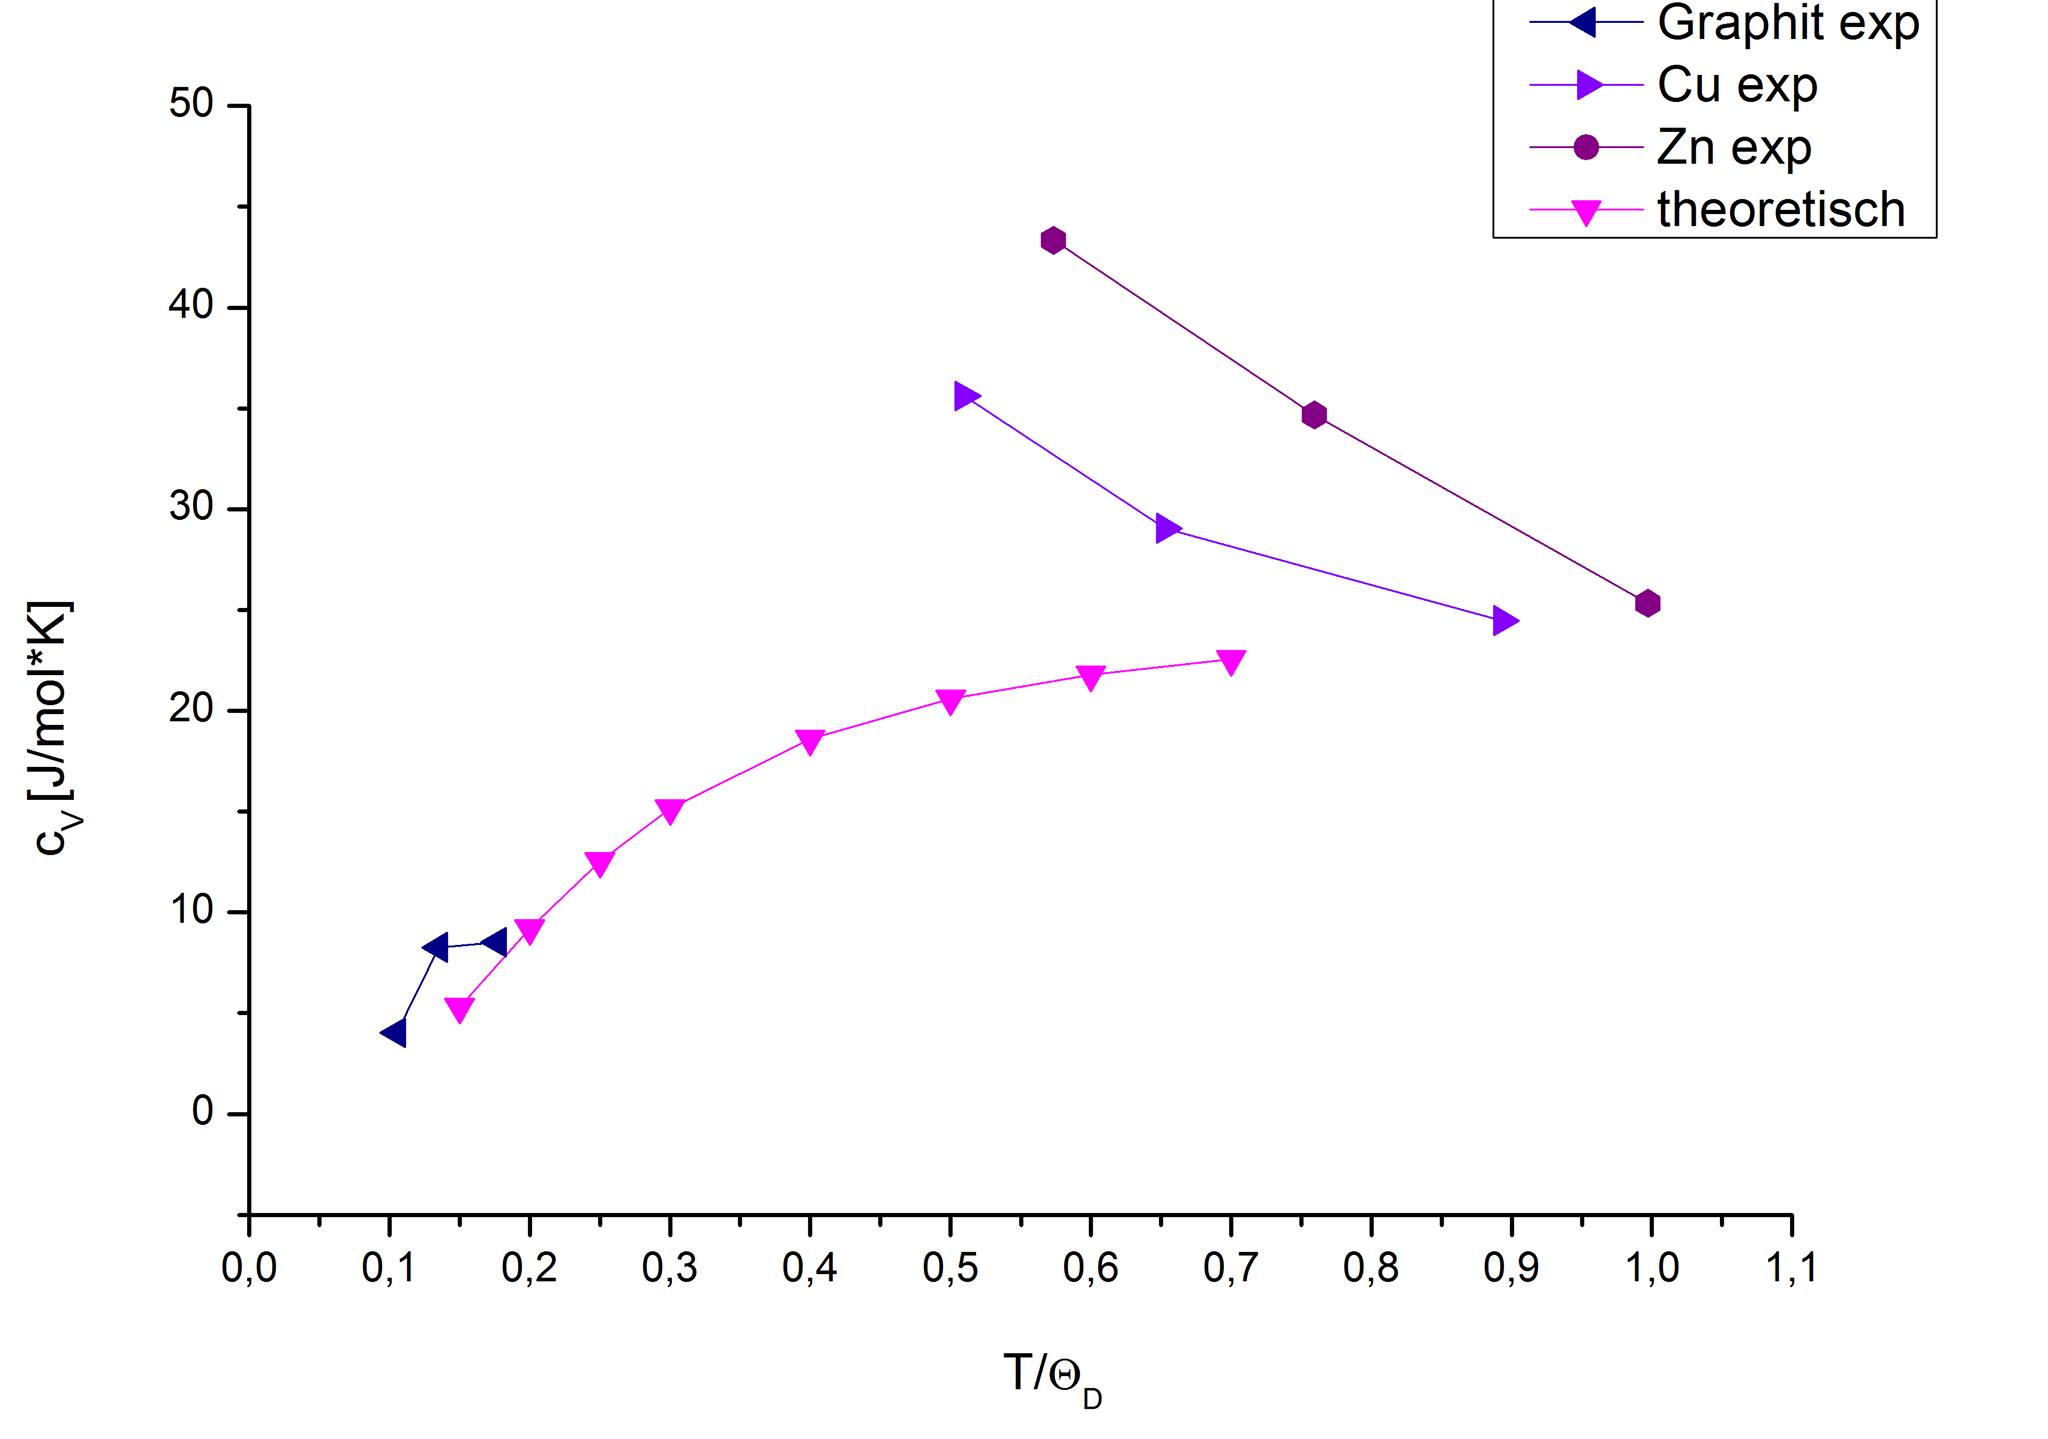
\includegraphics[width=13.5cm]{SUMM.jpeg}
\caption{Auftragung $\text{c}_V$ gegen $\frac{T}{\Theta_D}$.}
\end{figure}
\FloatBarrier
\section{Diskussion}
\begin{table}[h!]
\centering
\caption{Ergebnisse des Versuchs.}
\begin{tabular}{c|c|c}
Probe& $<\Theta_D >$ [K]& $<\Theta_{D,Lit.}>$ [K] \\
\hline
Graphit &1326 ± 4 & 1725\\
\hline
Zink & 317$^*$ & 345\\
\hline
Kupfer & 552$^*$ &308\\
\end{tabular}
\caption*{* korrigierter Mittelwerte (siehe Diskussion).}
\end{table}
\FloatBarrier
Die Debye-Temperatur des Graphits ist dem Literaturwert nicht nahe. Sie liegt unter dem Literaturwert. Ursache hierfür könnte an zu groß bestimmten Wärmekapazitäten sein. In Abbildung\;2 ist zu erkennen, dass die Fehlerbalken recht groß sind. Wenn bei beiden aufgetragen Wärmekapazitäten der wahre Wert der Wärmekapazität auf dem unteren Teil der Balken angenommen wird, würde die Gerade des $c_V$-Werts den Graphen bei einer höheren Temperatur schneiden. Diese Verschiebung wäre plausible durch zu klein bestimmte Temperaturdifferenzen. Die Wärmekapazität bei größer bestimmten Temperaturdifferenzen wäre nach Gl.\;1 kleiner. Daraus würde die Verschiebung auf der y-Achse in der Abbildung\;2 folgen. Diese zu kleine bestimmte Temperaturdifferenzen könnte, da die Wärmeisolierung nicht ideal ist, durch die Abgabe von Heizenergie an die Umgebung verursacht sein. \\
Aus den Graphen des Kupfers und Zinks konnte keine Debye-Temperatur bestimmt werden. Da die Ergebnisse eine Zunahme der Wärmekapazität mit sinkender Temperatur bedeuten würden und dies aus physikalischer Sicht unsinnig ist, wird  zum einen die der Korrekturfaktor als Ursache für die Abweichung in Frage kommen. Es wird bei der Korrektur angenommen, dass die Abweichung der experimentell bestimmten Wärmekapazitäten auch bei tieferen Temperaturen durch den Korrekturfaktor kompensiert wird. Wenn dieser Ansatz fehlschlägt und die Abweichung der Messungen bei tieferen Temperaturen größer sind, ist bei einer Korrektur des Korrekturfaktors um 0,2 ist insgesamt eine positive Steigung aus den Graphen ablesbar. Diese Ergebnisse sind physikalisch plausible. Die Abbildungen\;6 und 7 zeigen die Korrekturen bei Kupfer und Zink. Der Mittelwert der Debye-Temperature liegt für Kupfer bei 552\;K und für Zink bei 317\;K. Im Vergleich zur bestimmten Debye-Temperatur des Graphits liegen diese unter Tausend Kelvin, was den Trend der Literaturwerte wiederspiegelt und die Theorie zu groß bestimmten Korrekturfaktors unterstützen würde. Zum Anderen könnte bei diesem Experiementen auch aufgrund nicht idealer Wärmeisolierung Heizenergie an die Umgebung angegeben worden sein. Das würde zu zu geringen Temperaturdifferenzen führen, was bei sehr hoher Abgabe an die Umgebung die Verschiebung der Wärmekapazität nach oben auf der y-Achse verursachen würde. 
\begin{figure}
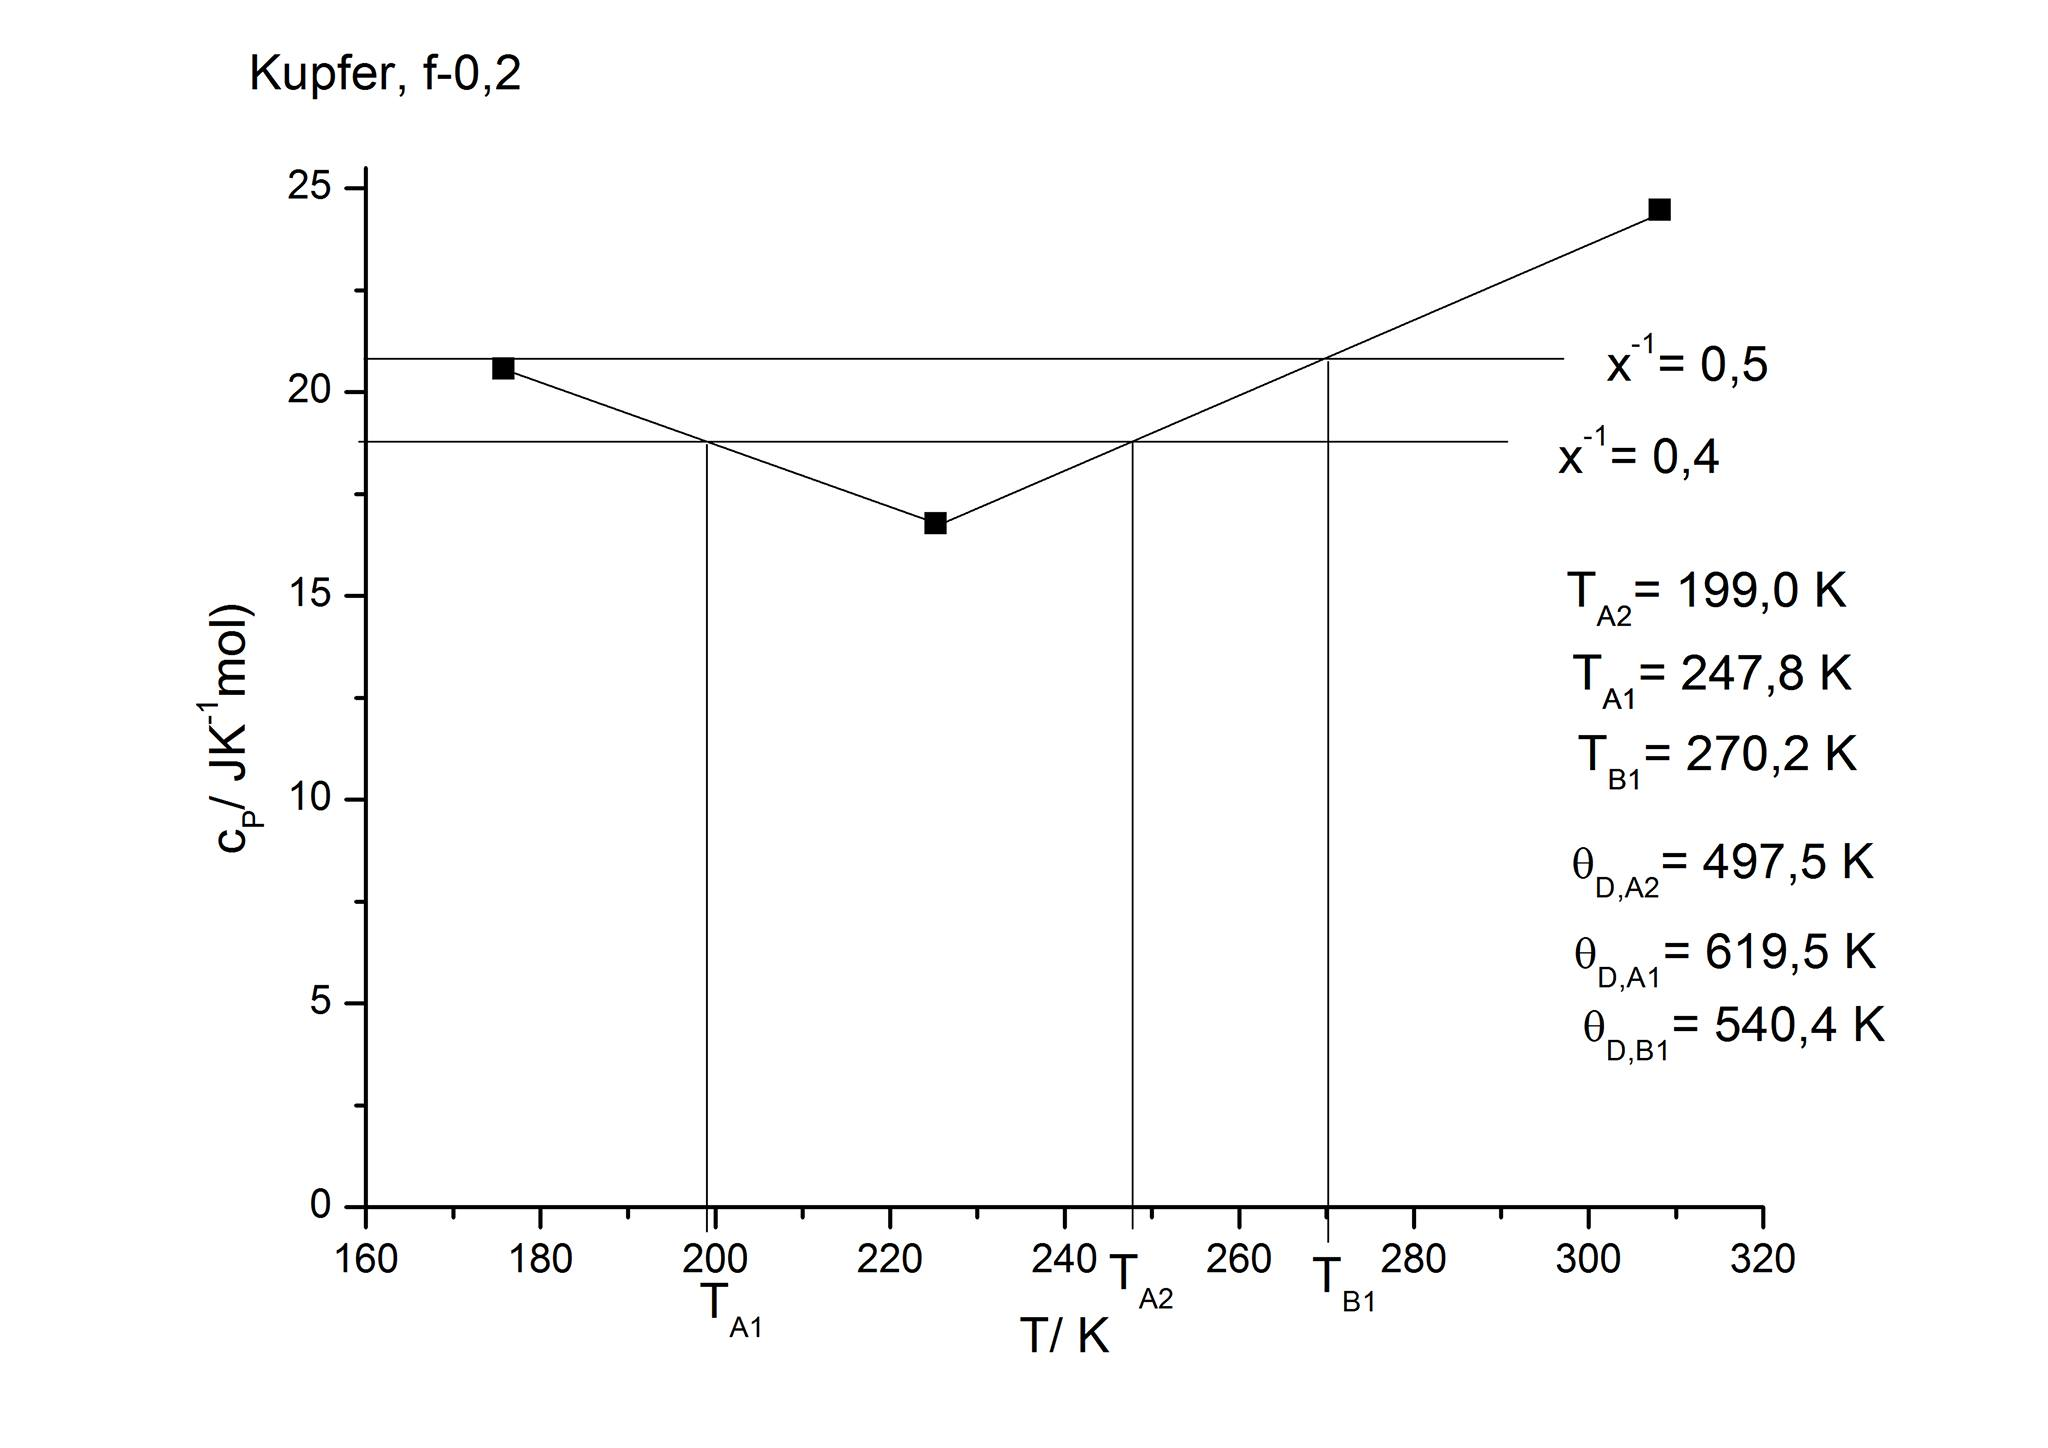
\includegraphics[width=13.5cm]{Cu_02.jpeg}
\caption{$c_P(T)$ und berechnete Debye-Temperaturen (Kupfer), Korrektur des Korrekturfaktors um 0,2.}
\end{figure}
\FloatBarrier
\begin{figure}
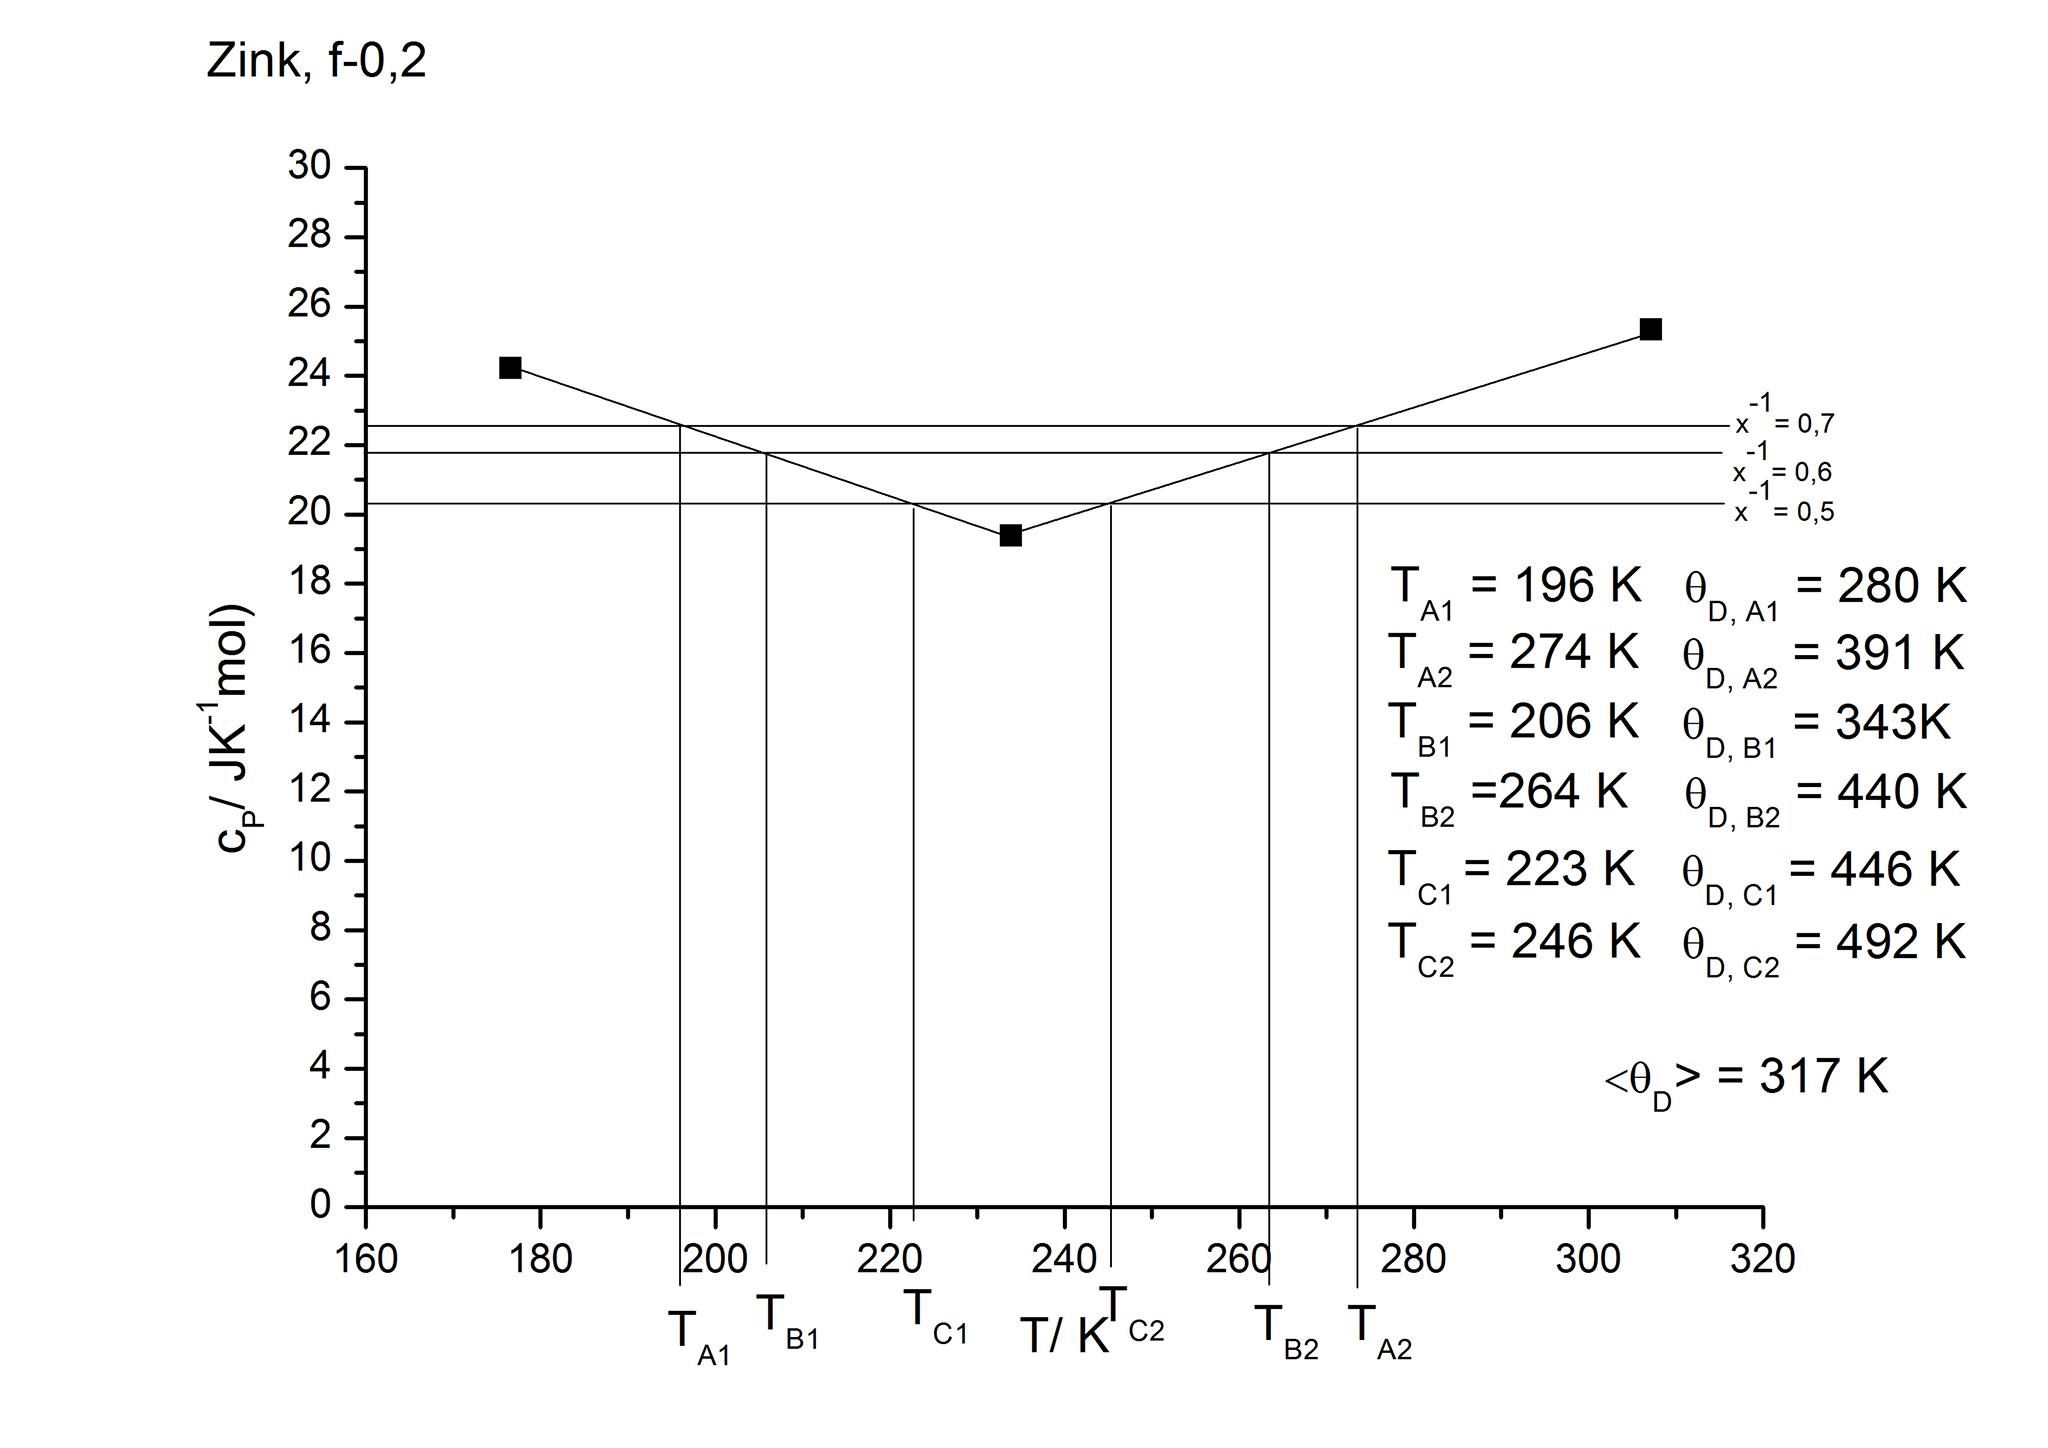
\includegraphics[width=13.5cm]{Zn_02.jpeg}
\caption{$c_P(T)$ und berechnete Debye-Temperaturen (Zink), Korrektur des Korrekturfaktors um 0,2.}
\end{figure}
\FloatBarrier
%Die experimentell bestimmten Wärmekapazitäten sind dem Literaturwert nicht nahe. Die Wärmekapazität von Graphit liegt unter dem Literaturwert. Ursache hierfür könnte in der Bestimmung der Temperaturdifferenz liegen. Die zu große Temperaturdifferenz führt zu einem Nenner im Quotienten aus Gl. 1, sodass die berechnete Wärmekapazität zu kleiner als die tatsächliche Wärmekapazität ist. Die Wärmekapazitäten für Zink und Kupfer liegen um einen Faktor 2 über dem Literaturwert. Ursache hierfür könnte bei Kupfer die Temperaturabhänigkeit sein. Kupfer ist, wie an Abbildungen 3 zu erkennen ist, stärker temperaturabhängig, sodass die nicht SATP-Bedingungen zu einer großen Abweichung vom Literaturwert führen könnte. \\
%Die berechneten Mittelwerte der Debytemperaturen sind den jeweiligen Literaturwerten nicht nahe. Die berechnete Debye-Temperatur bei Graphit liegt um einen Faktor über $10^2$ unter dem Literaturwert. Ursache könnte die Steigung m aus der Auftragung sein. Ist die Steigung zu groß, ist das Ergebniss für die Temperatur zu klein, sodasss die berechnete Debye-Temperatur zu klein ist. Die Steigung könnte aufgrund der zu kleinen Wärmekapazität bei Raumtemperatur zu groß sein. Wie schon diskutiert, könnte die zu geringe Wärmekapazität an der zu groß bestimmten Temperaturdifferenzen liegen. Die Debye-Temperaturen von Zink und Kupfer liegen um einen Fator von mehr als 2 über den Literaturwerten. Bei der Auswertung von Zink konnte die Messung bei Stickstoff/Ethanol-Bad nicht ausgewertet werden. Die zwei Messpunkte könnten eine Ursache für die große Ungenauigkeit sein. Des Weiteren könnte eine Ursache für die positive Abweichung könnte beim Zink die geringe Steigung m sein. Hier durch wird der Quotient größer zur Berechnung der Temperatur größer, was die zu große Debye-Temperatur zur Folge hat.
%Eine Ursache für die zu große Debye-Temperatur bei Kupfer könnte der negative Wert für n sein. 



\newpage


\subsection{Literaturverzeichnis}
1\quad Eckhold, Götz: \emph{Praktikum I zur Physikalischen Chemie}, Institut für Physikalische Chemie, Uni Göttingen, \textbf{2014}.
\vspace{0,5 cm}

2 \quad Eckhold, Götz: \emph{Statistische Thermodynamik}, Institut für Physikalische Chemie, Uni Göttingen, \textbf{2012}.

\vspace{0,5cm}

3 \quad Eckhold, Götz: \emph{Chemisches Gleichgewicht}, Institut für Physikalische Chemie, Uni Göttingen, \textbf{2015}.\\

\end{document}


